\renewcommand{\thesubsection}{\arabic{subsection}}
\setcounter{subsection}{2}
%\setcounter{figure}{0}
\tocless\subsubsection{Schlaganfall als Krankheitsbild}
\begin{figure}[H]
\centering
\includesvg[width=0.8\textwidth]{pics/Schlaganfall}
\caption{Schaubild zum FAST-Test}
\label{fig:fasttest}
\end{figure}

\setcounter{subsection}{3}
\setcounter{subsubsection}{0}
\tocless\subsubsection{Gamification}
\begin{figure}[H]
\centering
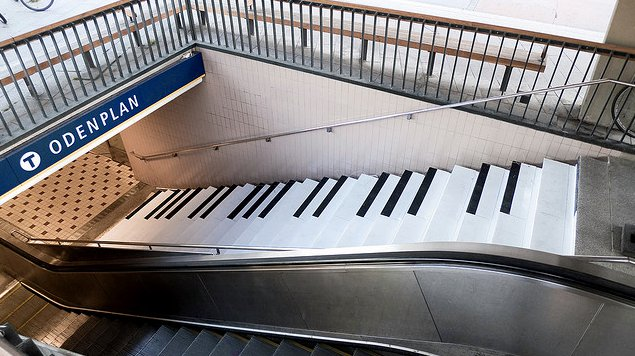
\includegraphics[width=0.8\textwidth]{pics/pianostairs.jpg}
\caption{Die Klavier-Treppe aus dem Projekt \emph{The Fun Theory}}
\label{fig:pianostairs}
\end{figure}


\setcounter{subsection}{4}
\setcounter{subsubsection}{0}
\tocless\subsubsection{Aufbau der Schaltung}
\begin{figure}[H]
	\centering
	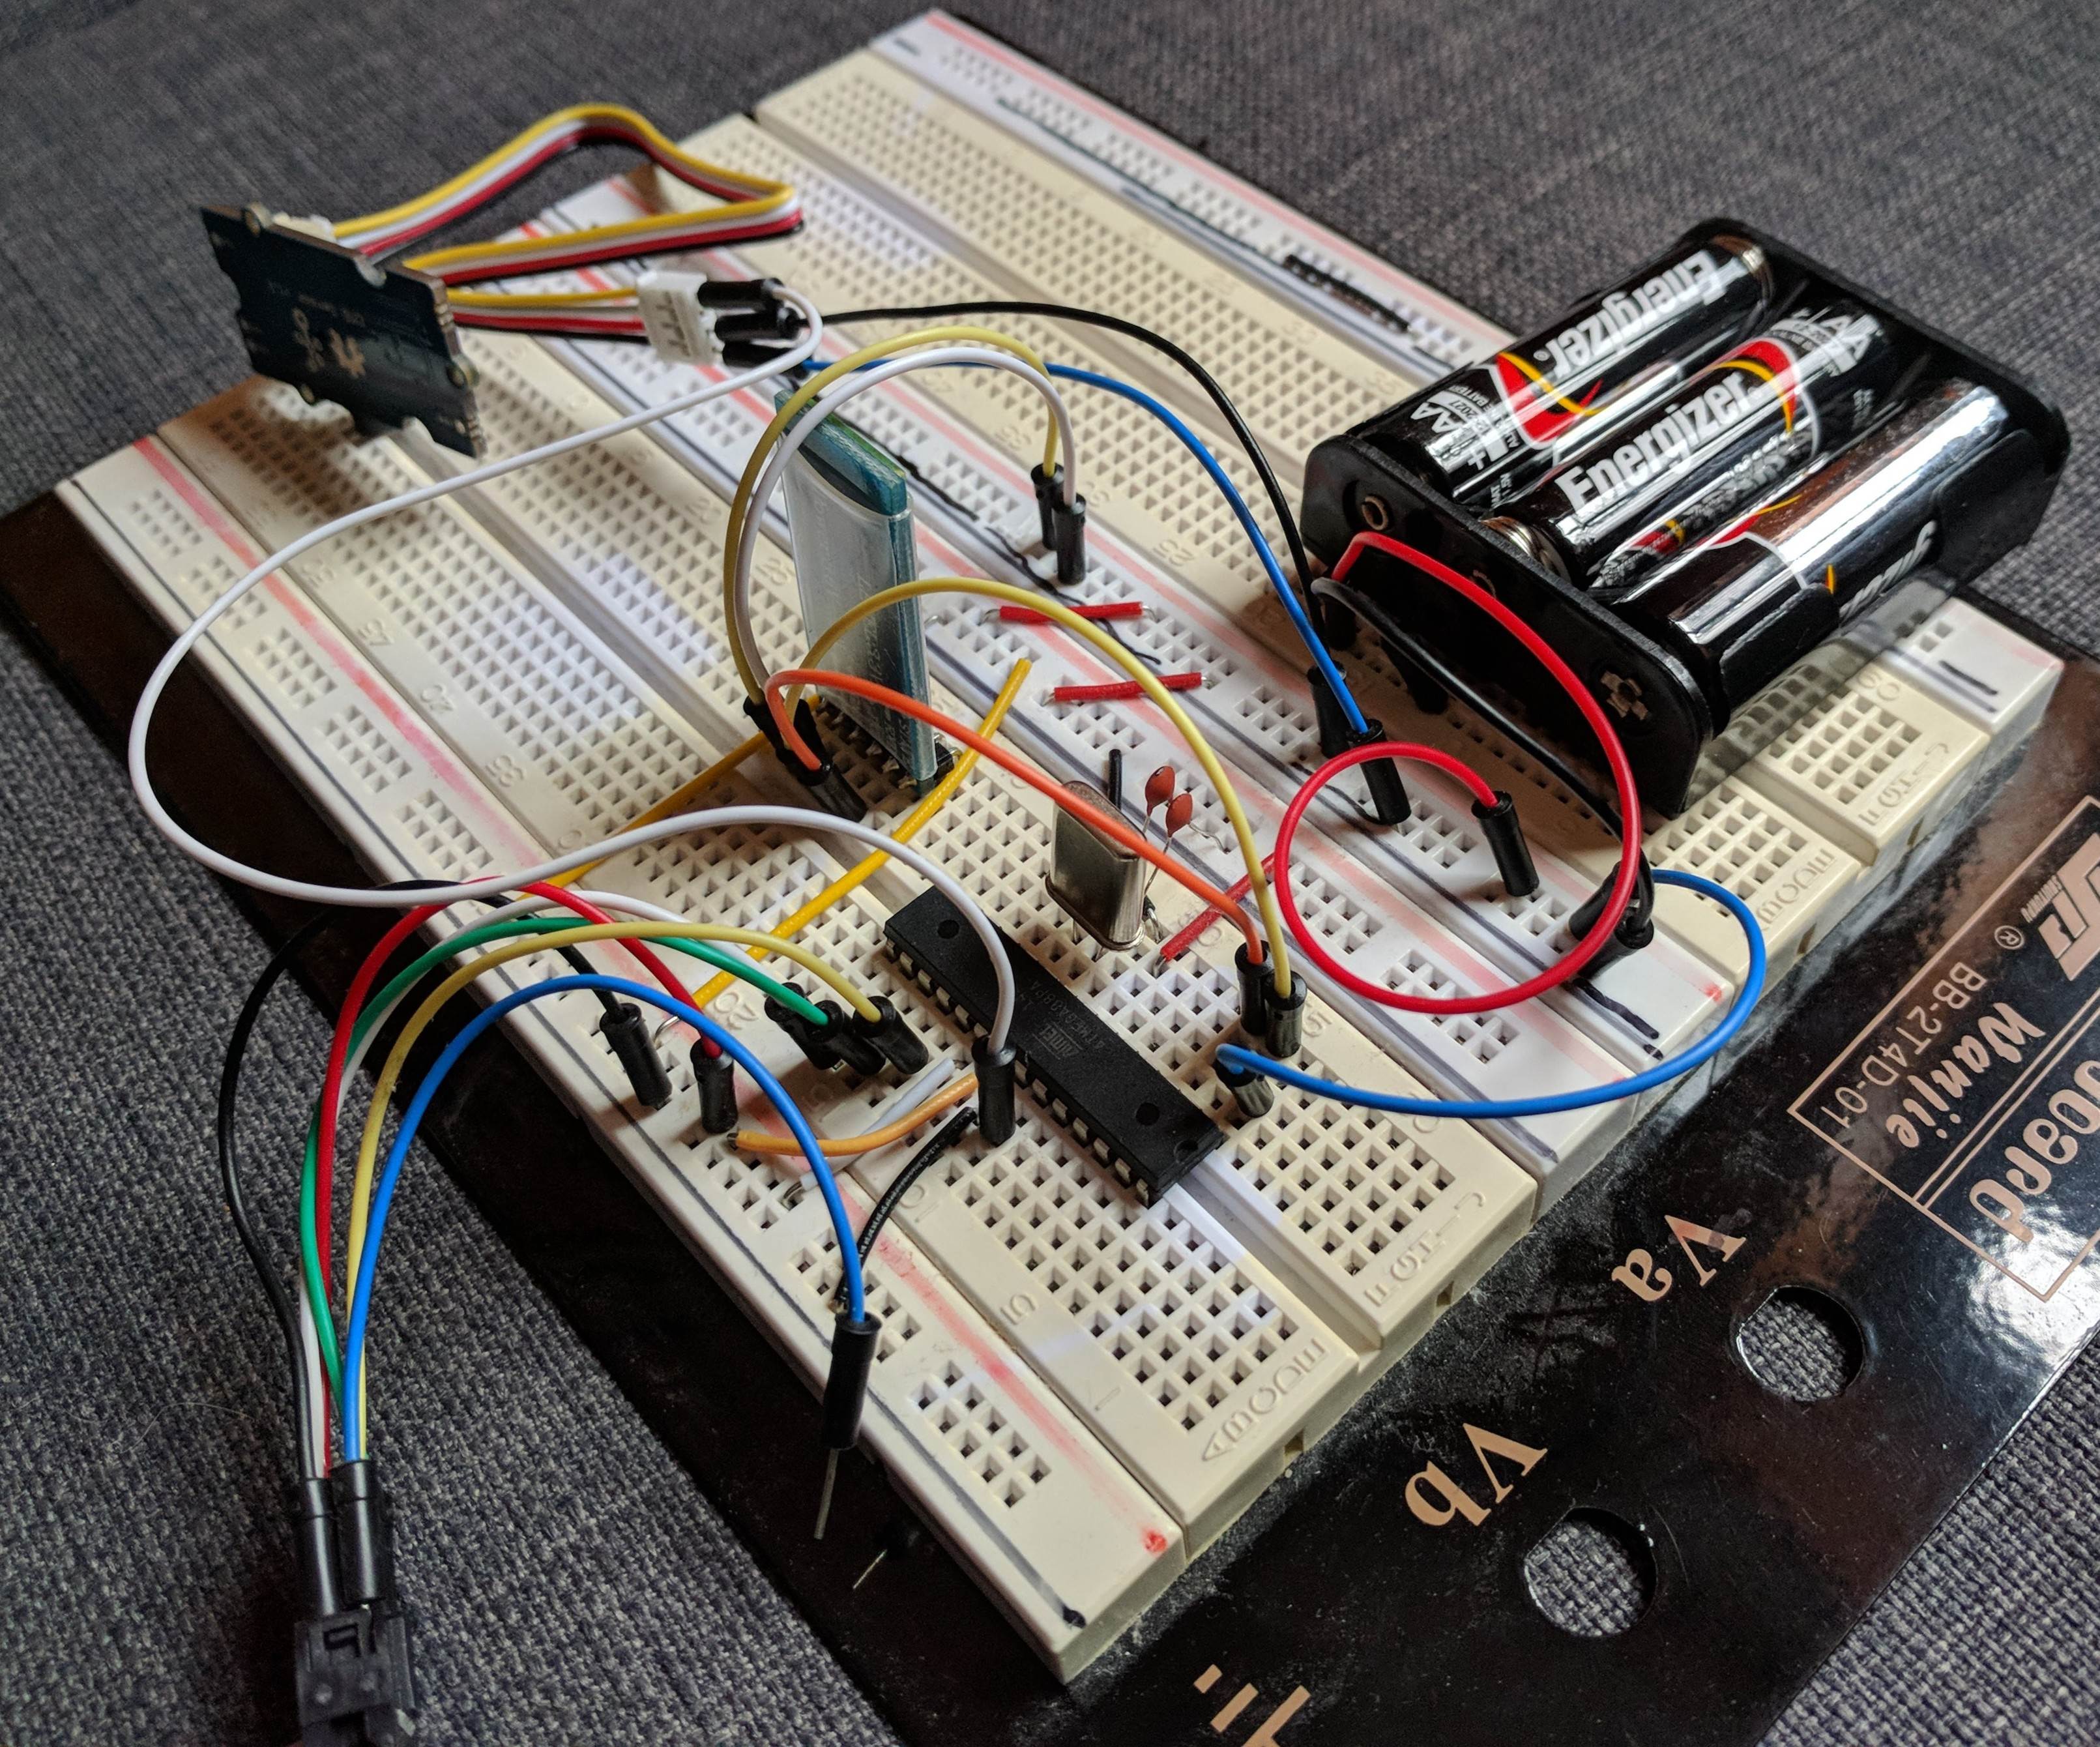
\includegraphics[width=0.7\textwidth]{pics/mikrocontroller.jpg}
	\caption{Foto der aufgebauten Schaltung auf einem Breadboard}
	\label{fig:mikrocon}
\end{figure}
\tocless\subsubsection{Entwicklung des Programms auf dem Mikrocontroller}
\renewcommand{\listingscaption}{Quellcode}
 \begin{longlisting}
 \cfile{../Softwareprodukt/Mikrocontroller/SchlaganfallRehaMotivationsGeraet/SchlaganfallRehaMotivationsGeraet/main.c}
 \caption{Das Programm für den Mikrocontroller}
 \label{listing:mikrocontroller}
 \end{longlisting}
 
\newpage
\setcounter{subsection}{5}
\setcounter{subsubsection}{0}
\tocless\subsubsection{Grundlegender Aufbau und Konzept der App}
\begin{multicols}{2}
\begin{figure}[H]
	\centering
	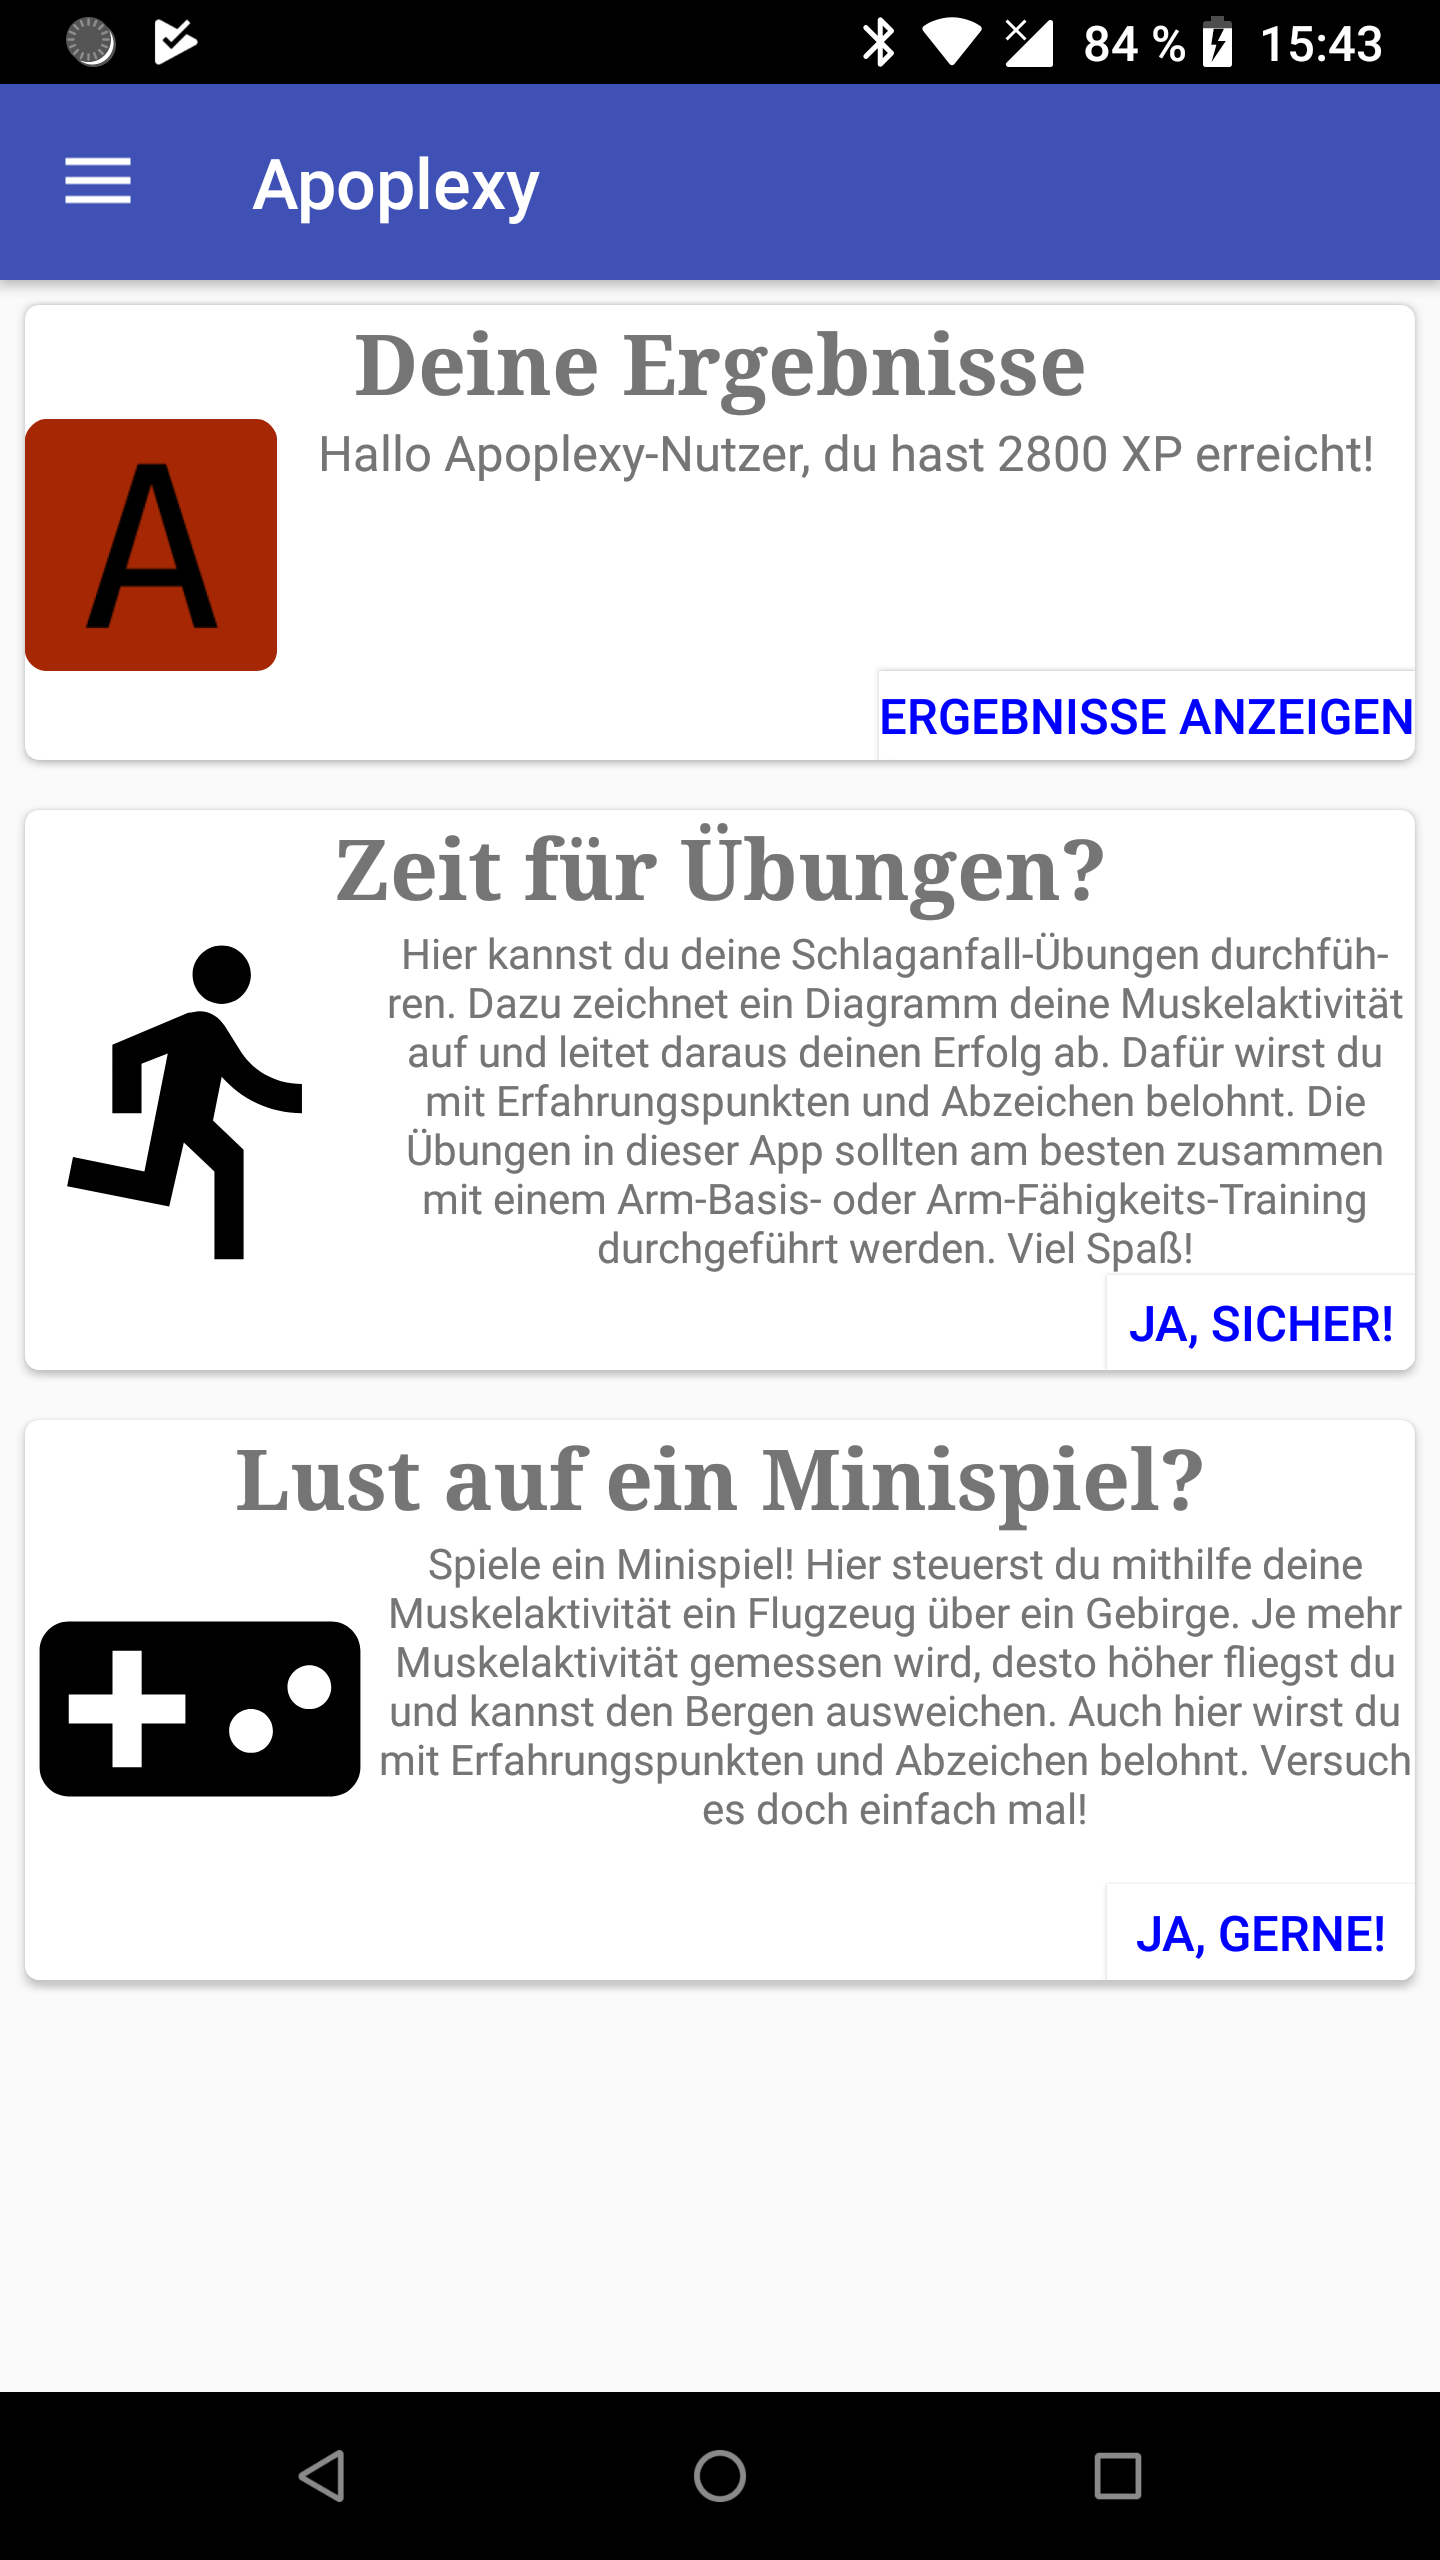
\includegraphics[scale=0.1]{pics/device-home.png}
	\caption{Die Startseite der App}
\end{figure}
\begin{figure}[H]
	\centering
	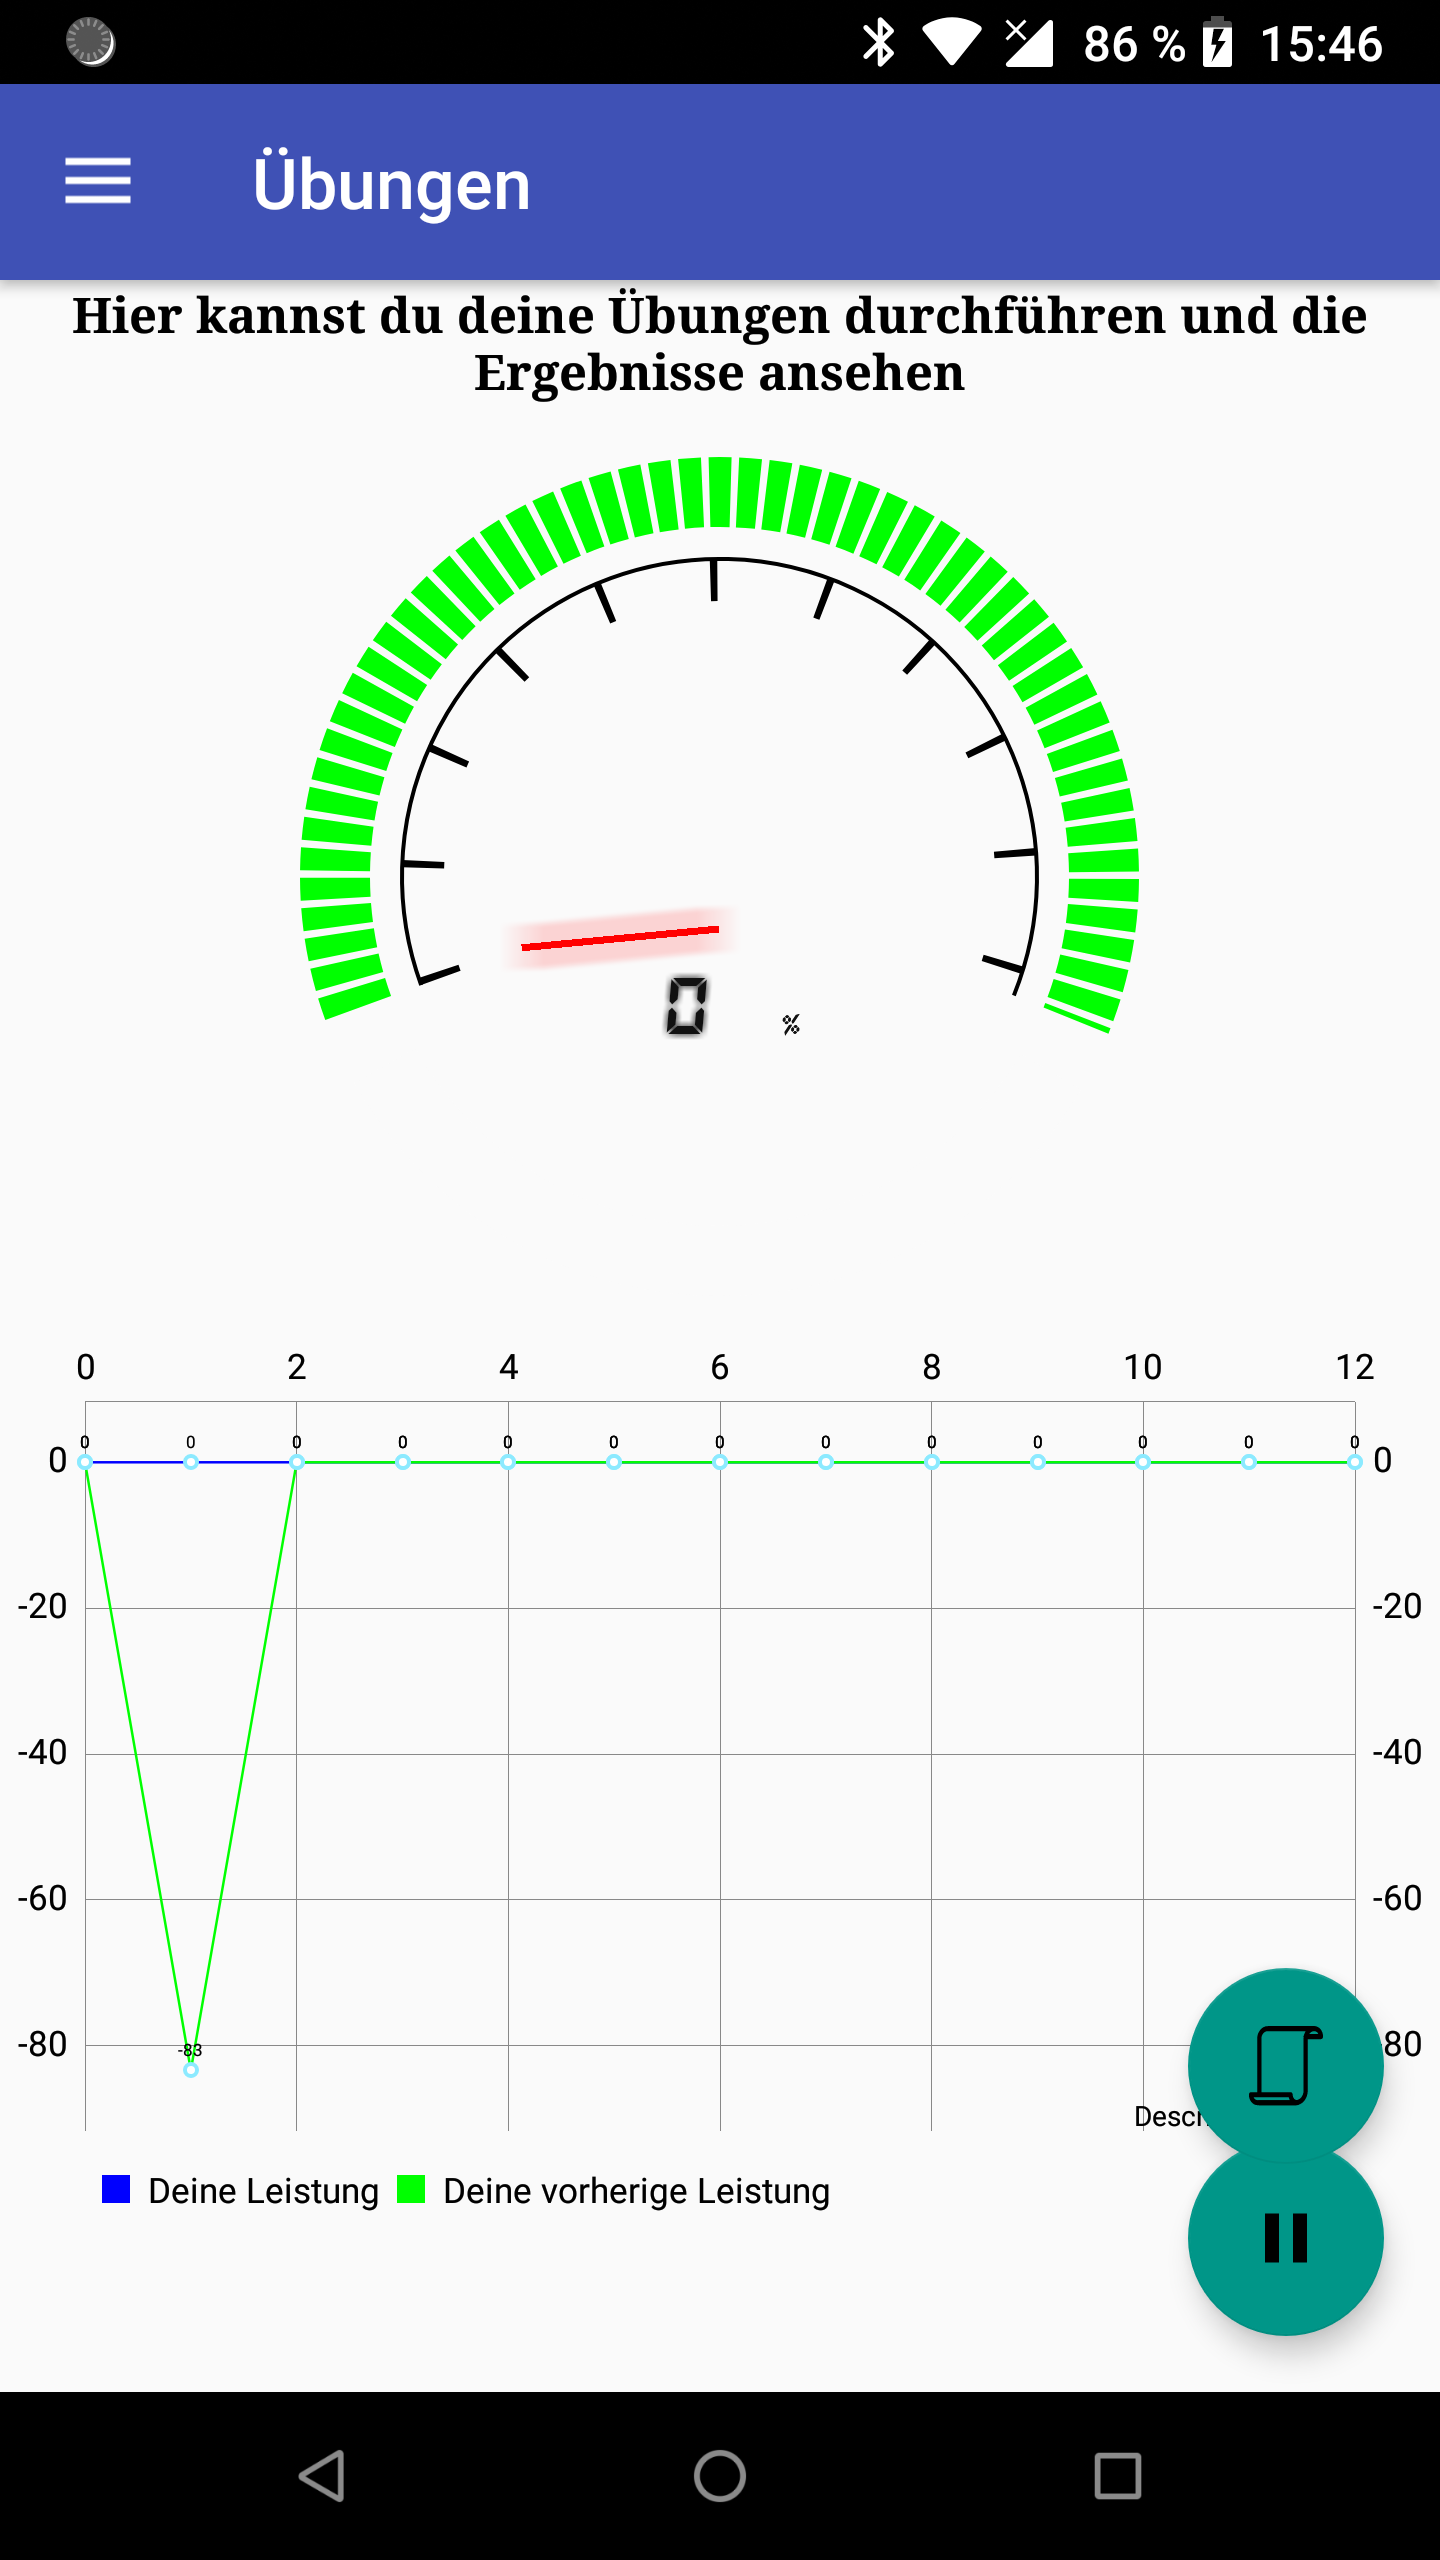
\includegraphics[scale=0.1]{pics/device-exercise.png}
	\caption{Die Übungsseite der App}
\end{figure}
\begin{figure}[H]
	\centering
	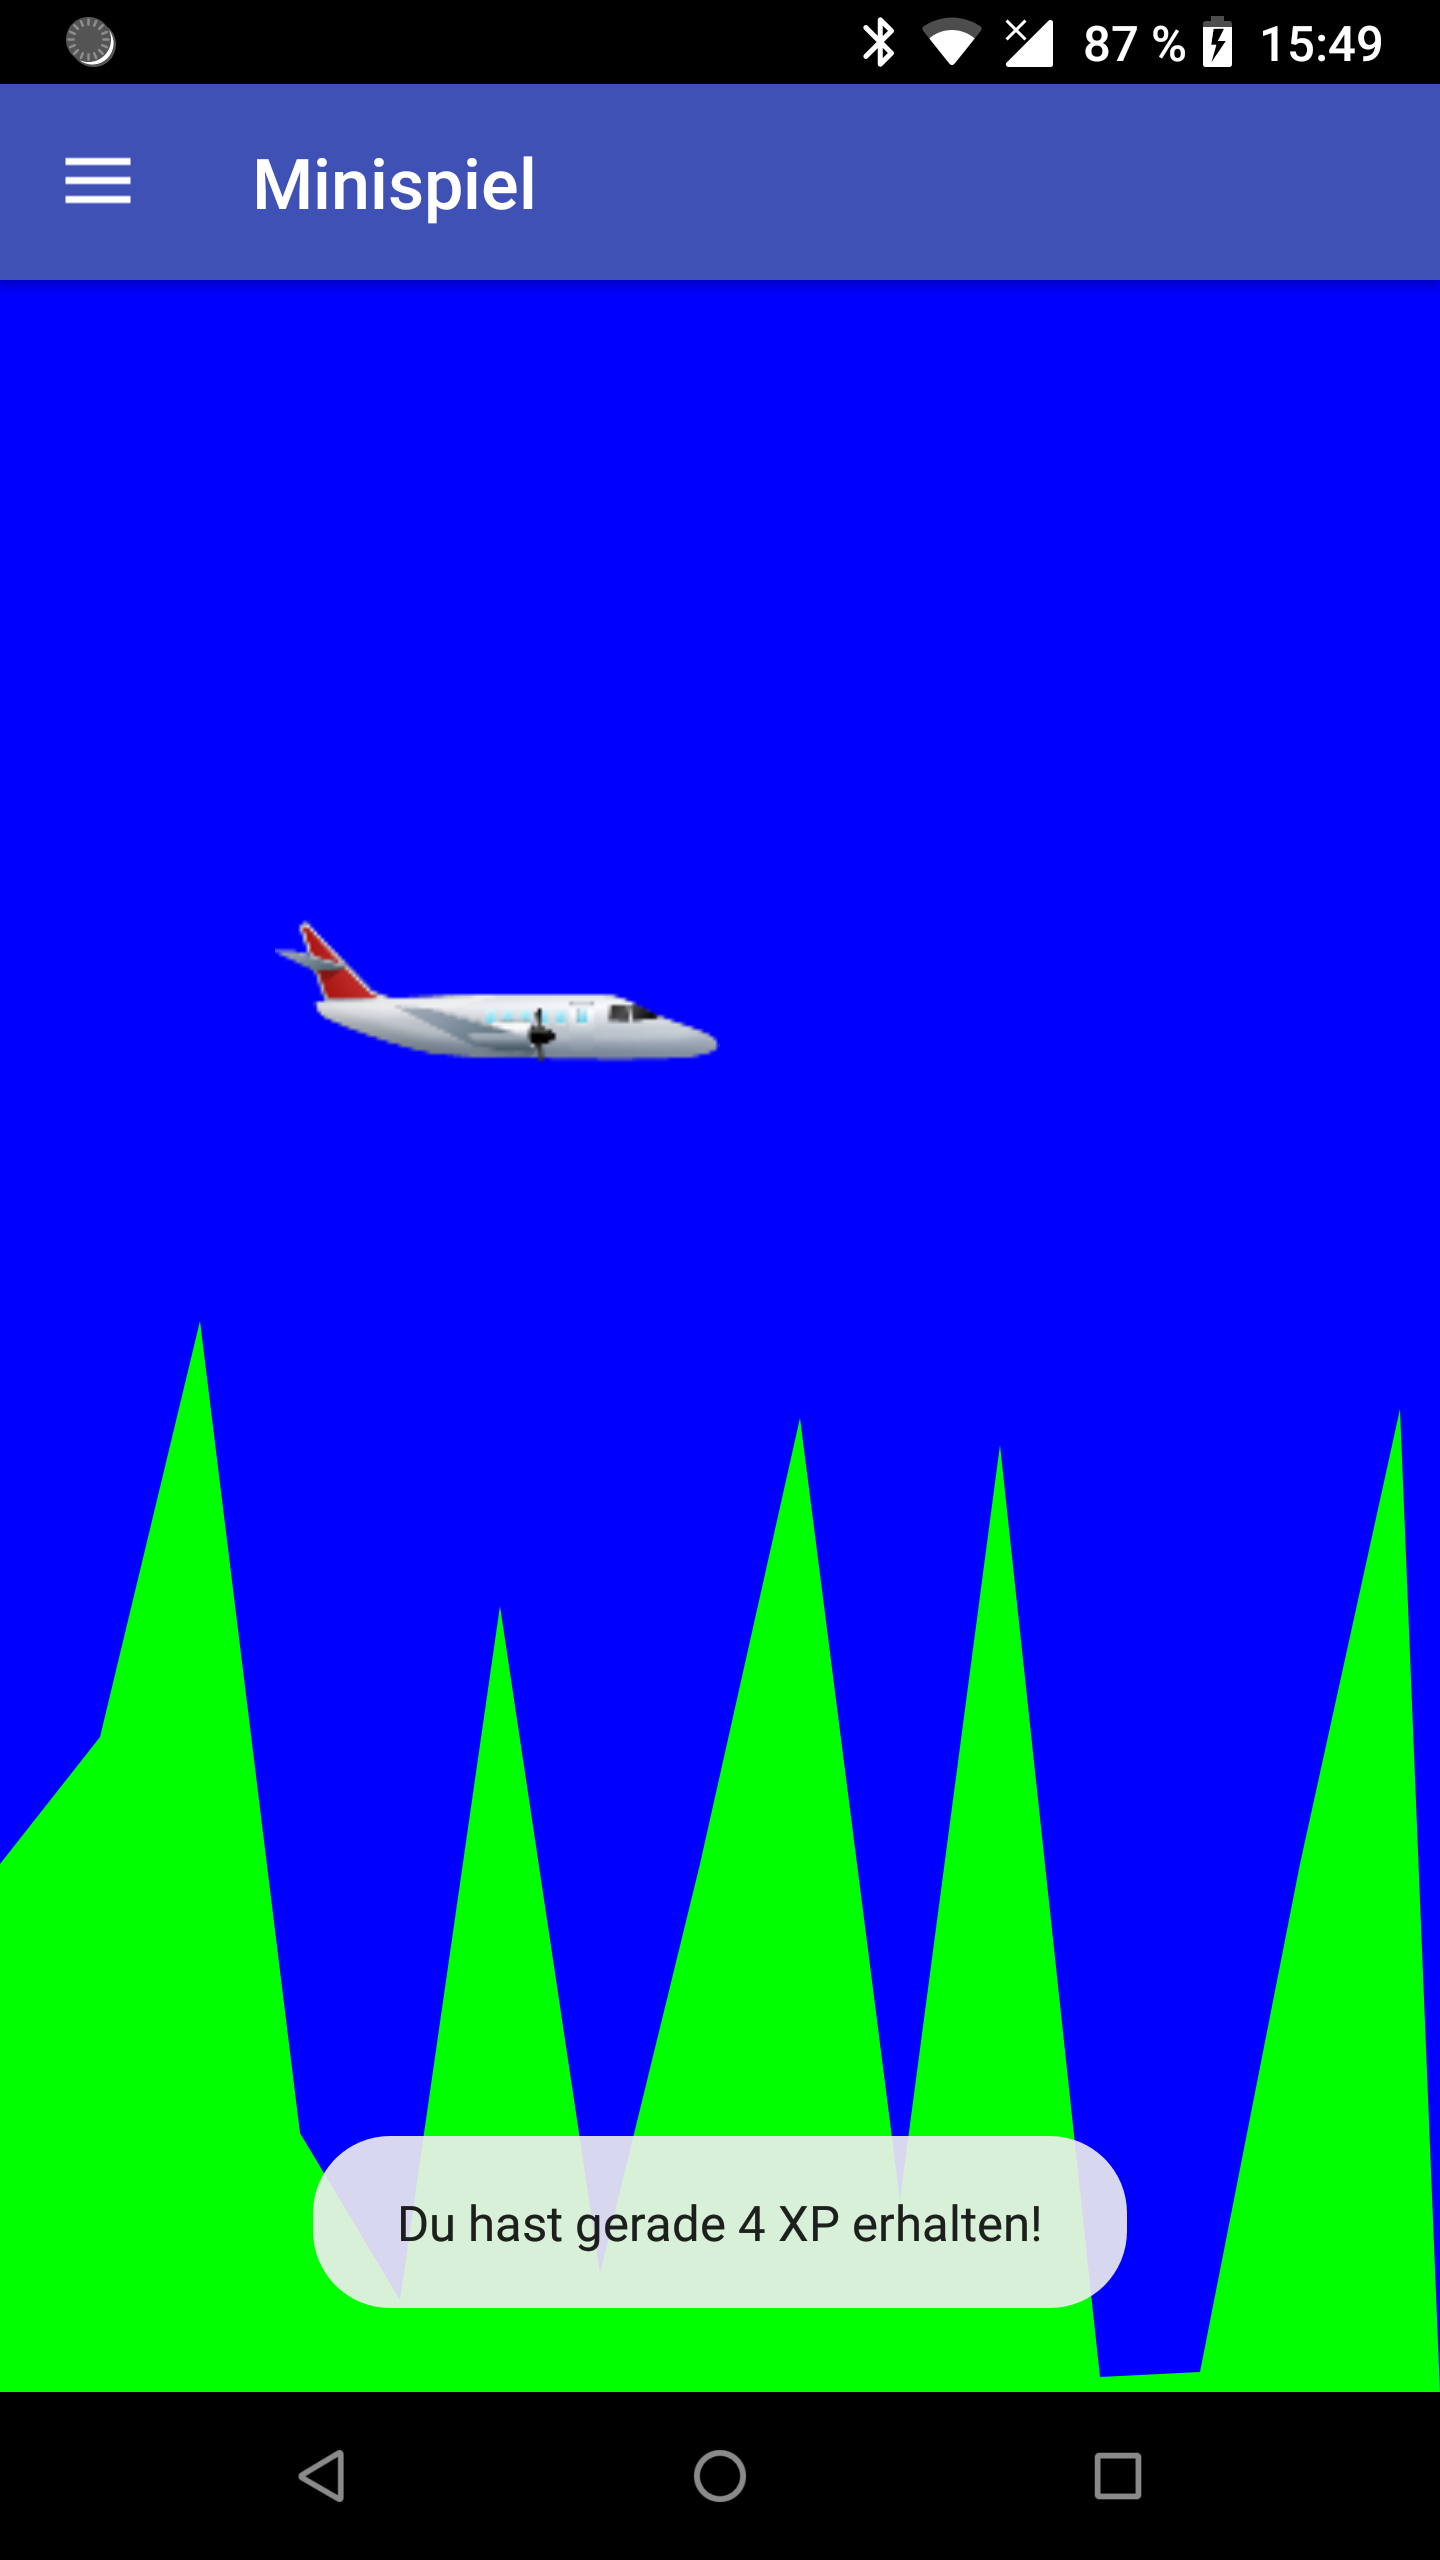
\includegraphics[scale=0.1]{pics/device-game.png}
	\caption{Das Minispiel}
\end{figure}
\begin{figure}[H]
	\centering
	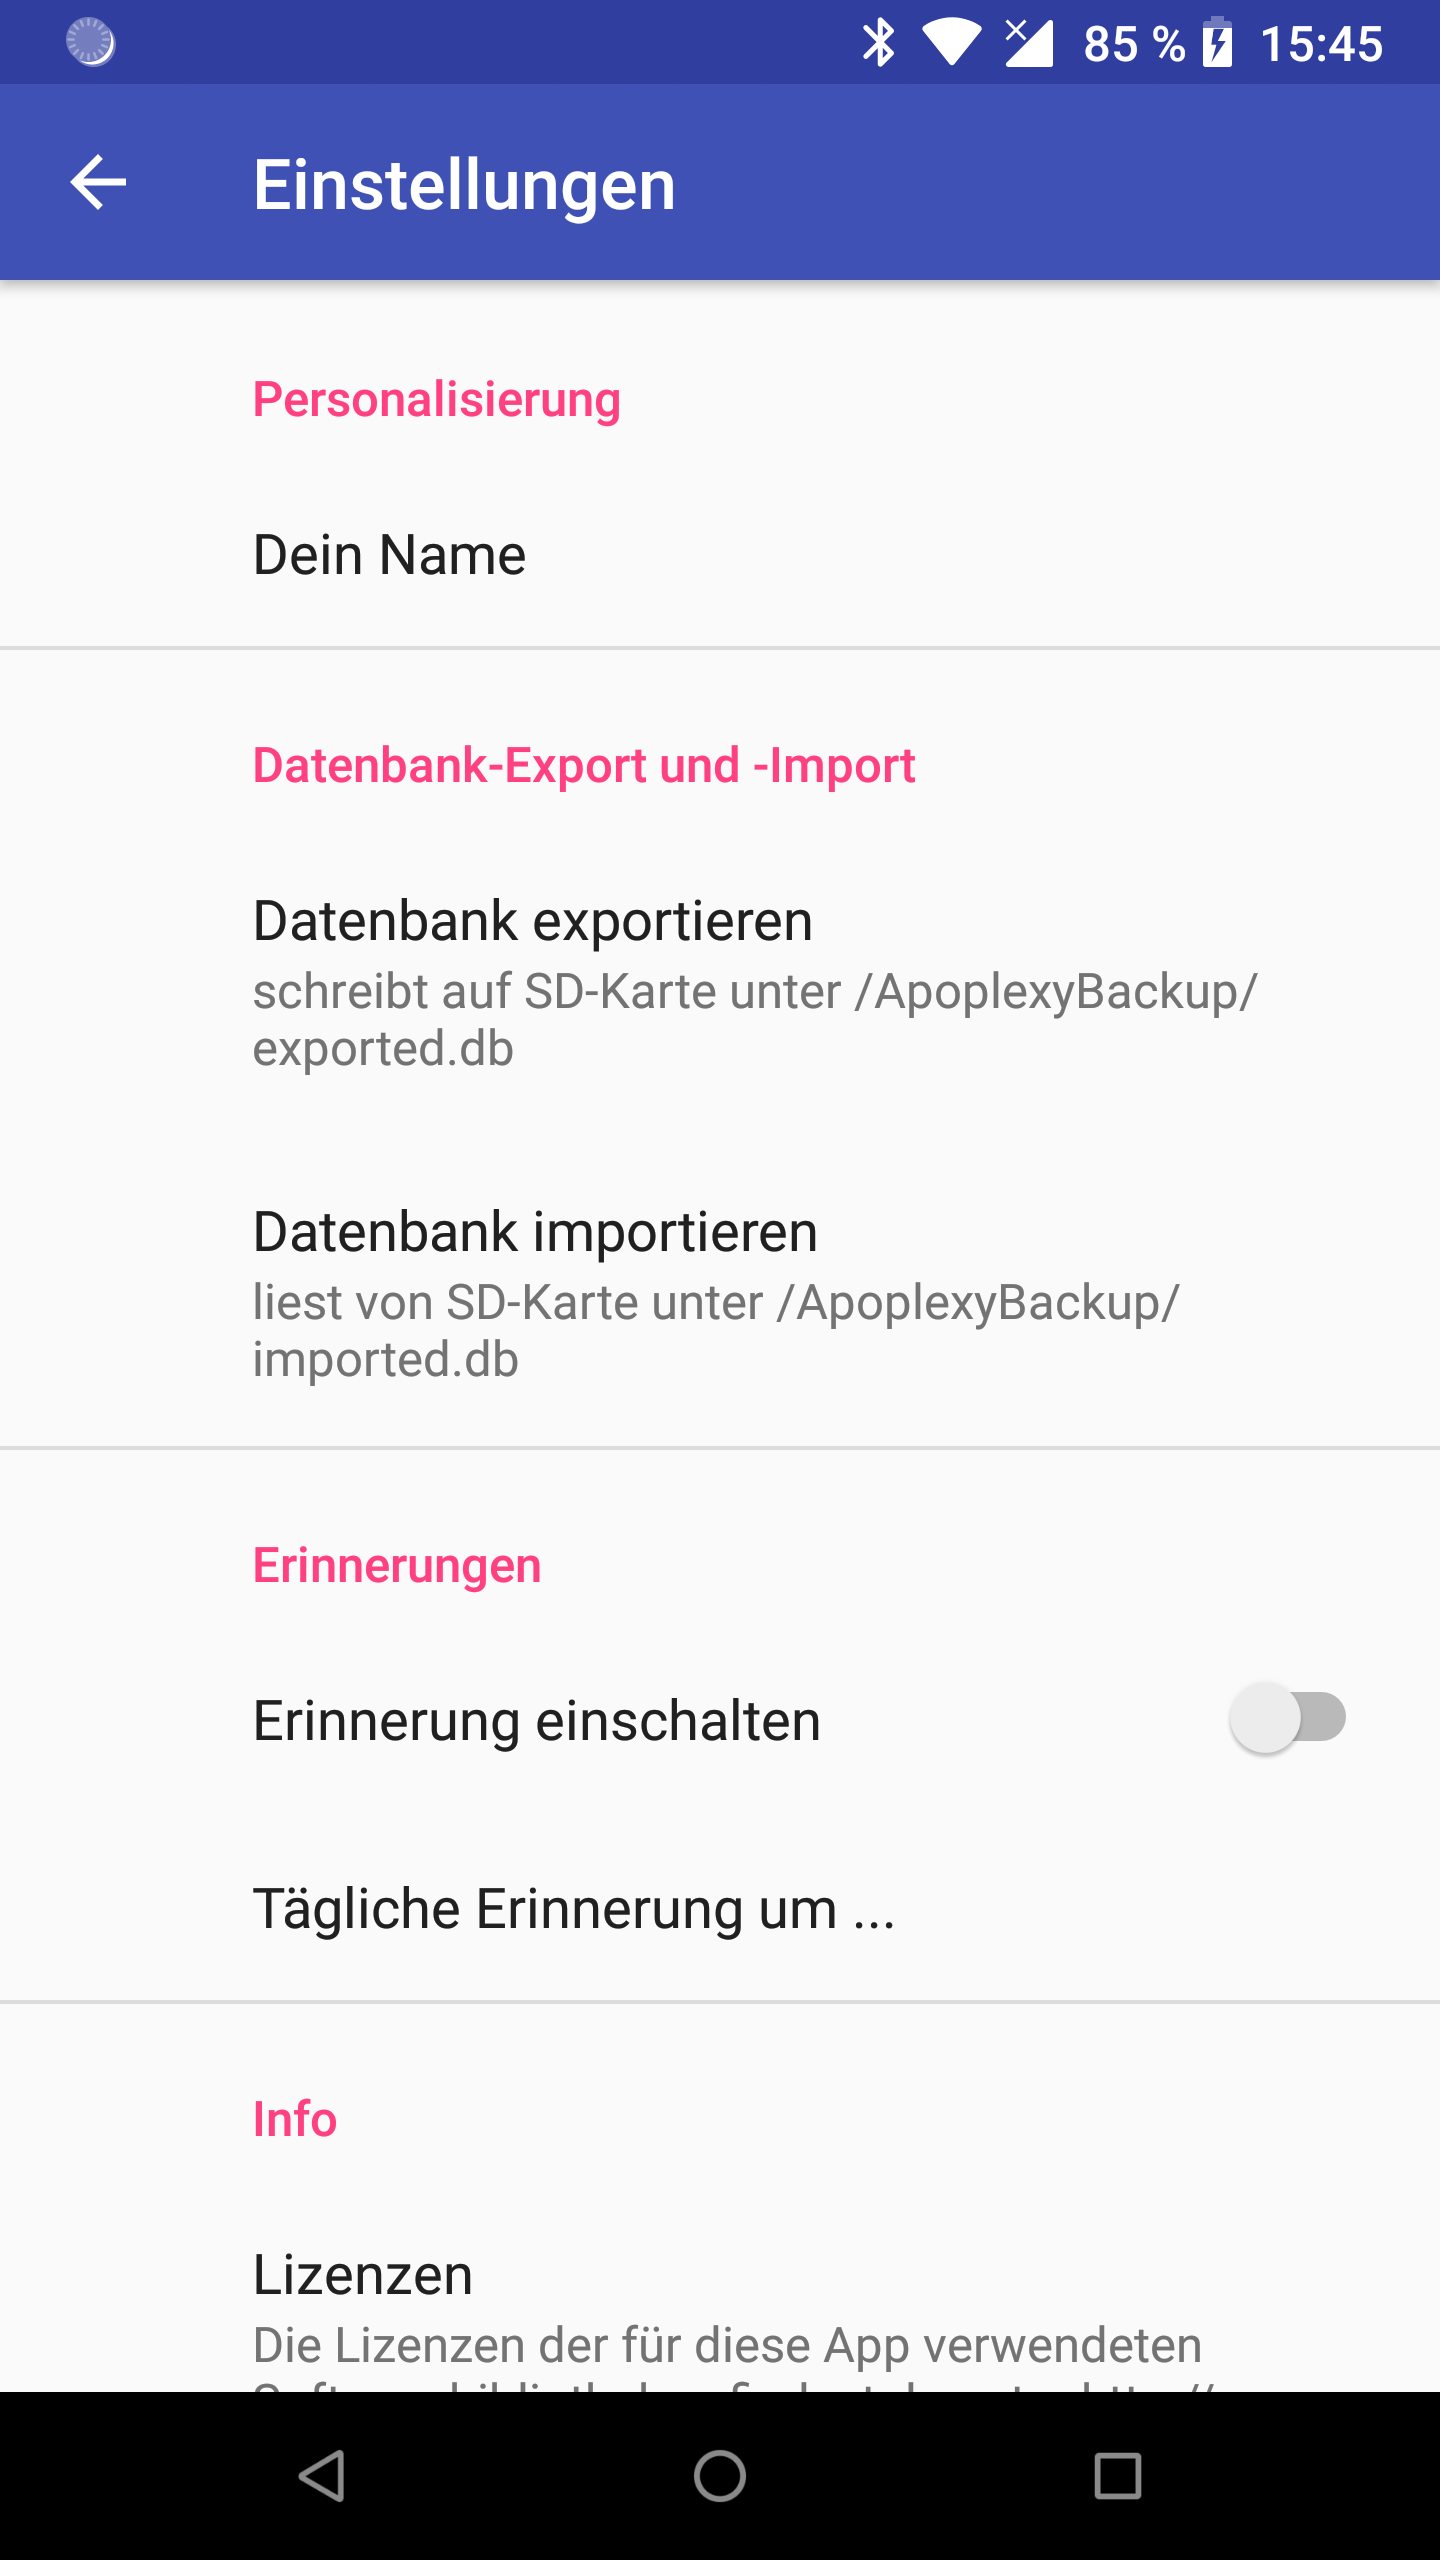
\includegraphics[scale=0.1]{pics/device-settings.png}
	\caption{Die Einstellungsseite der App}
\end{figure}
\begin{figure}[H]
	\centering
	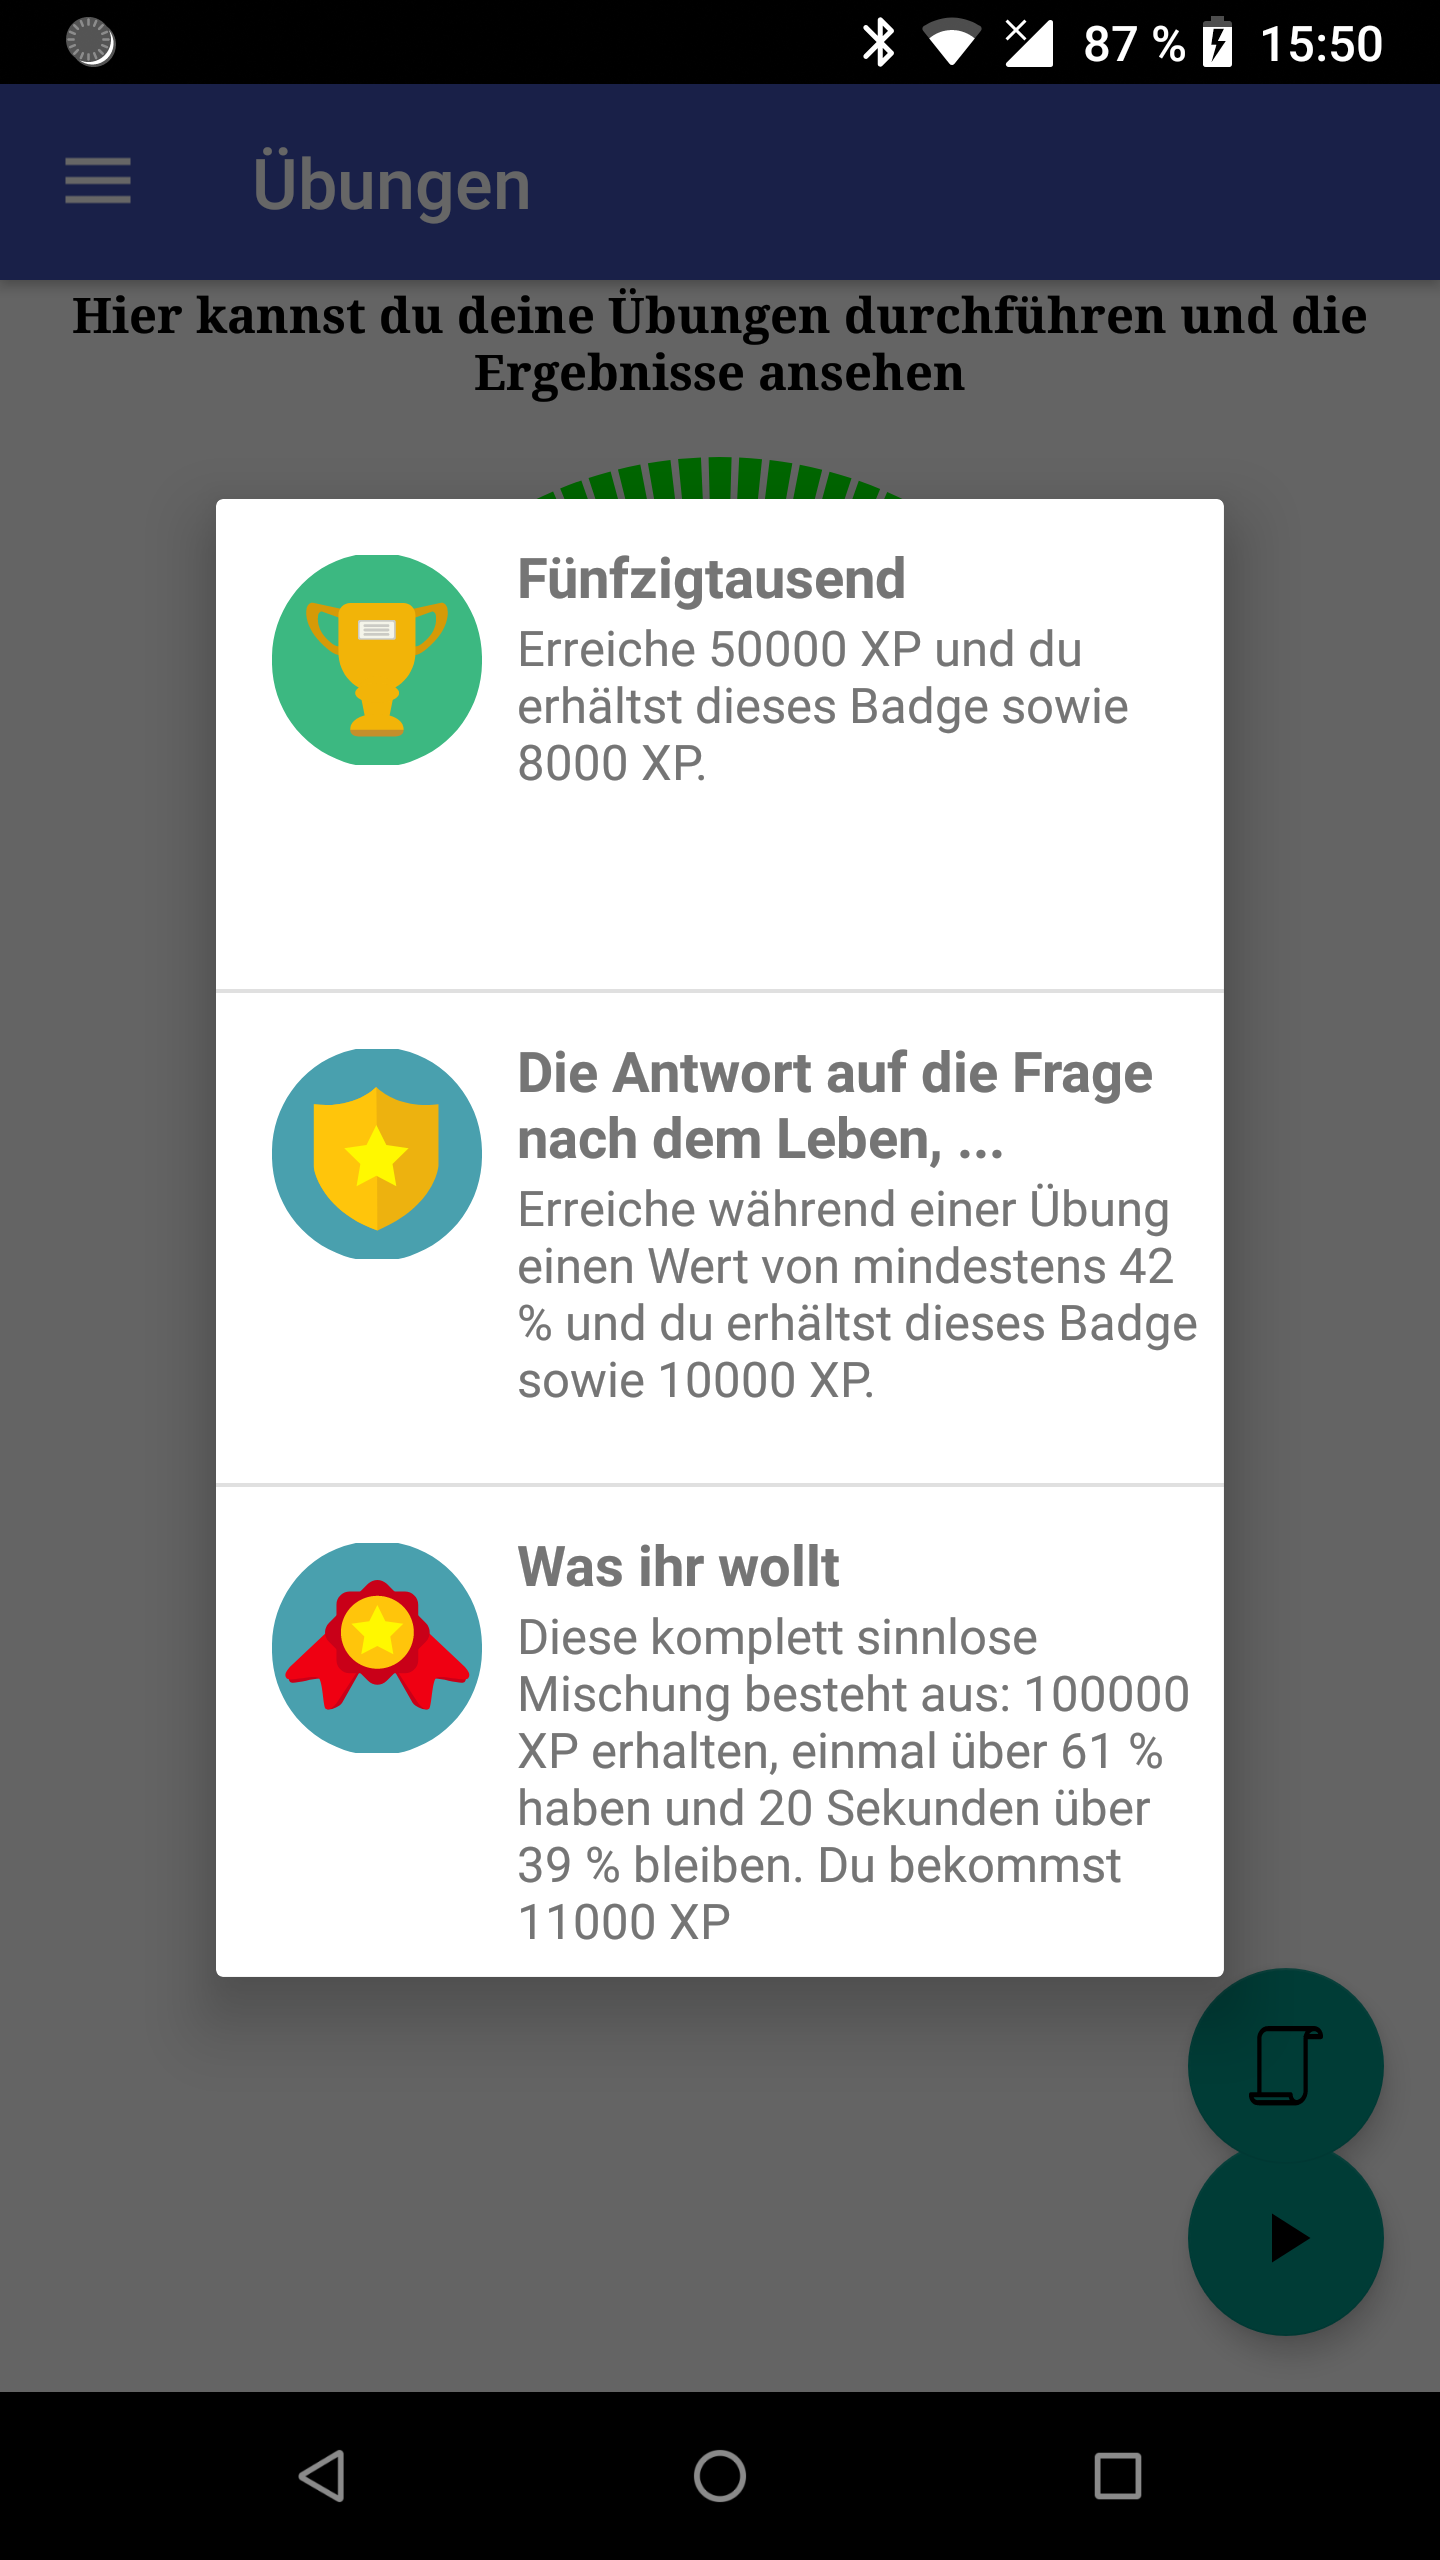
\includegraphics[scale=0.1]{pics/device-badges.png}
	\caption{Die Liste der verfügbaren Quests}
\end{figure}
\begin{figure}[H]
	\centering
	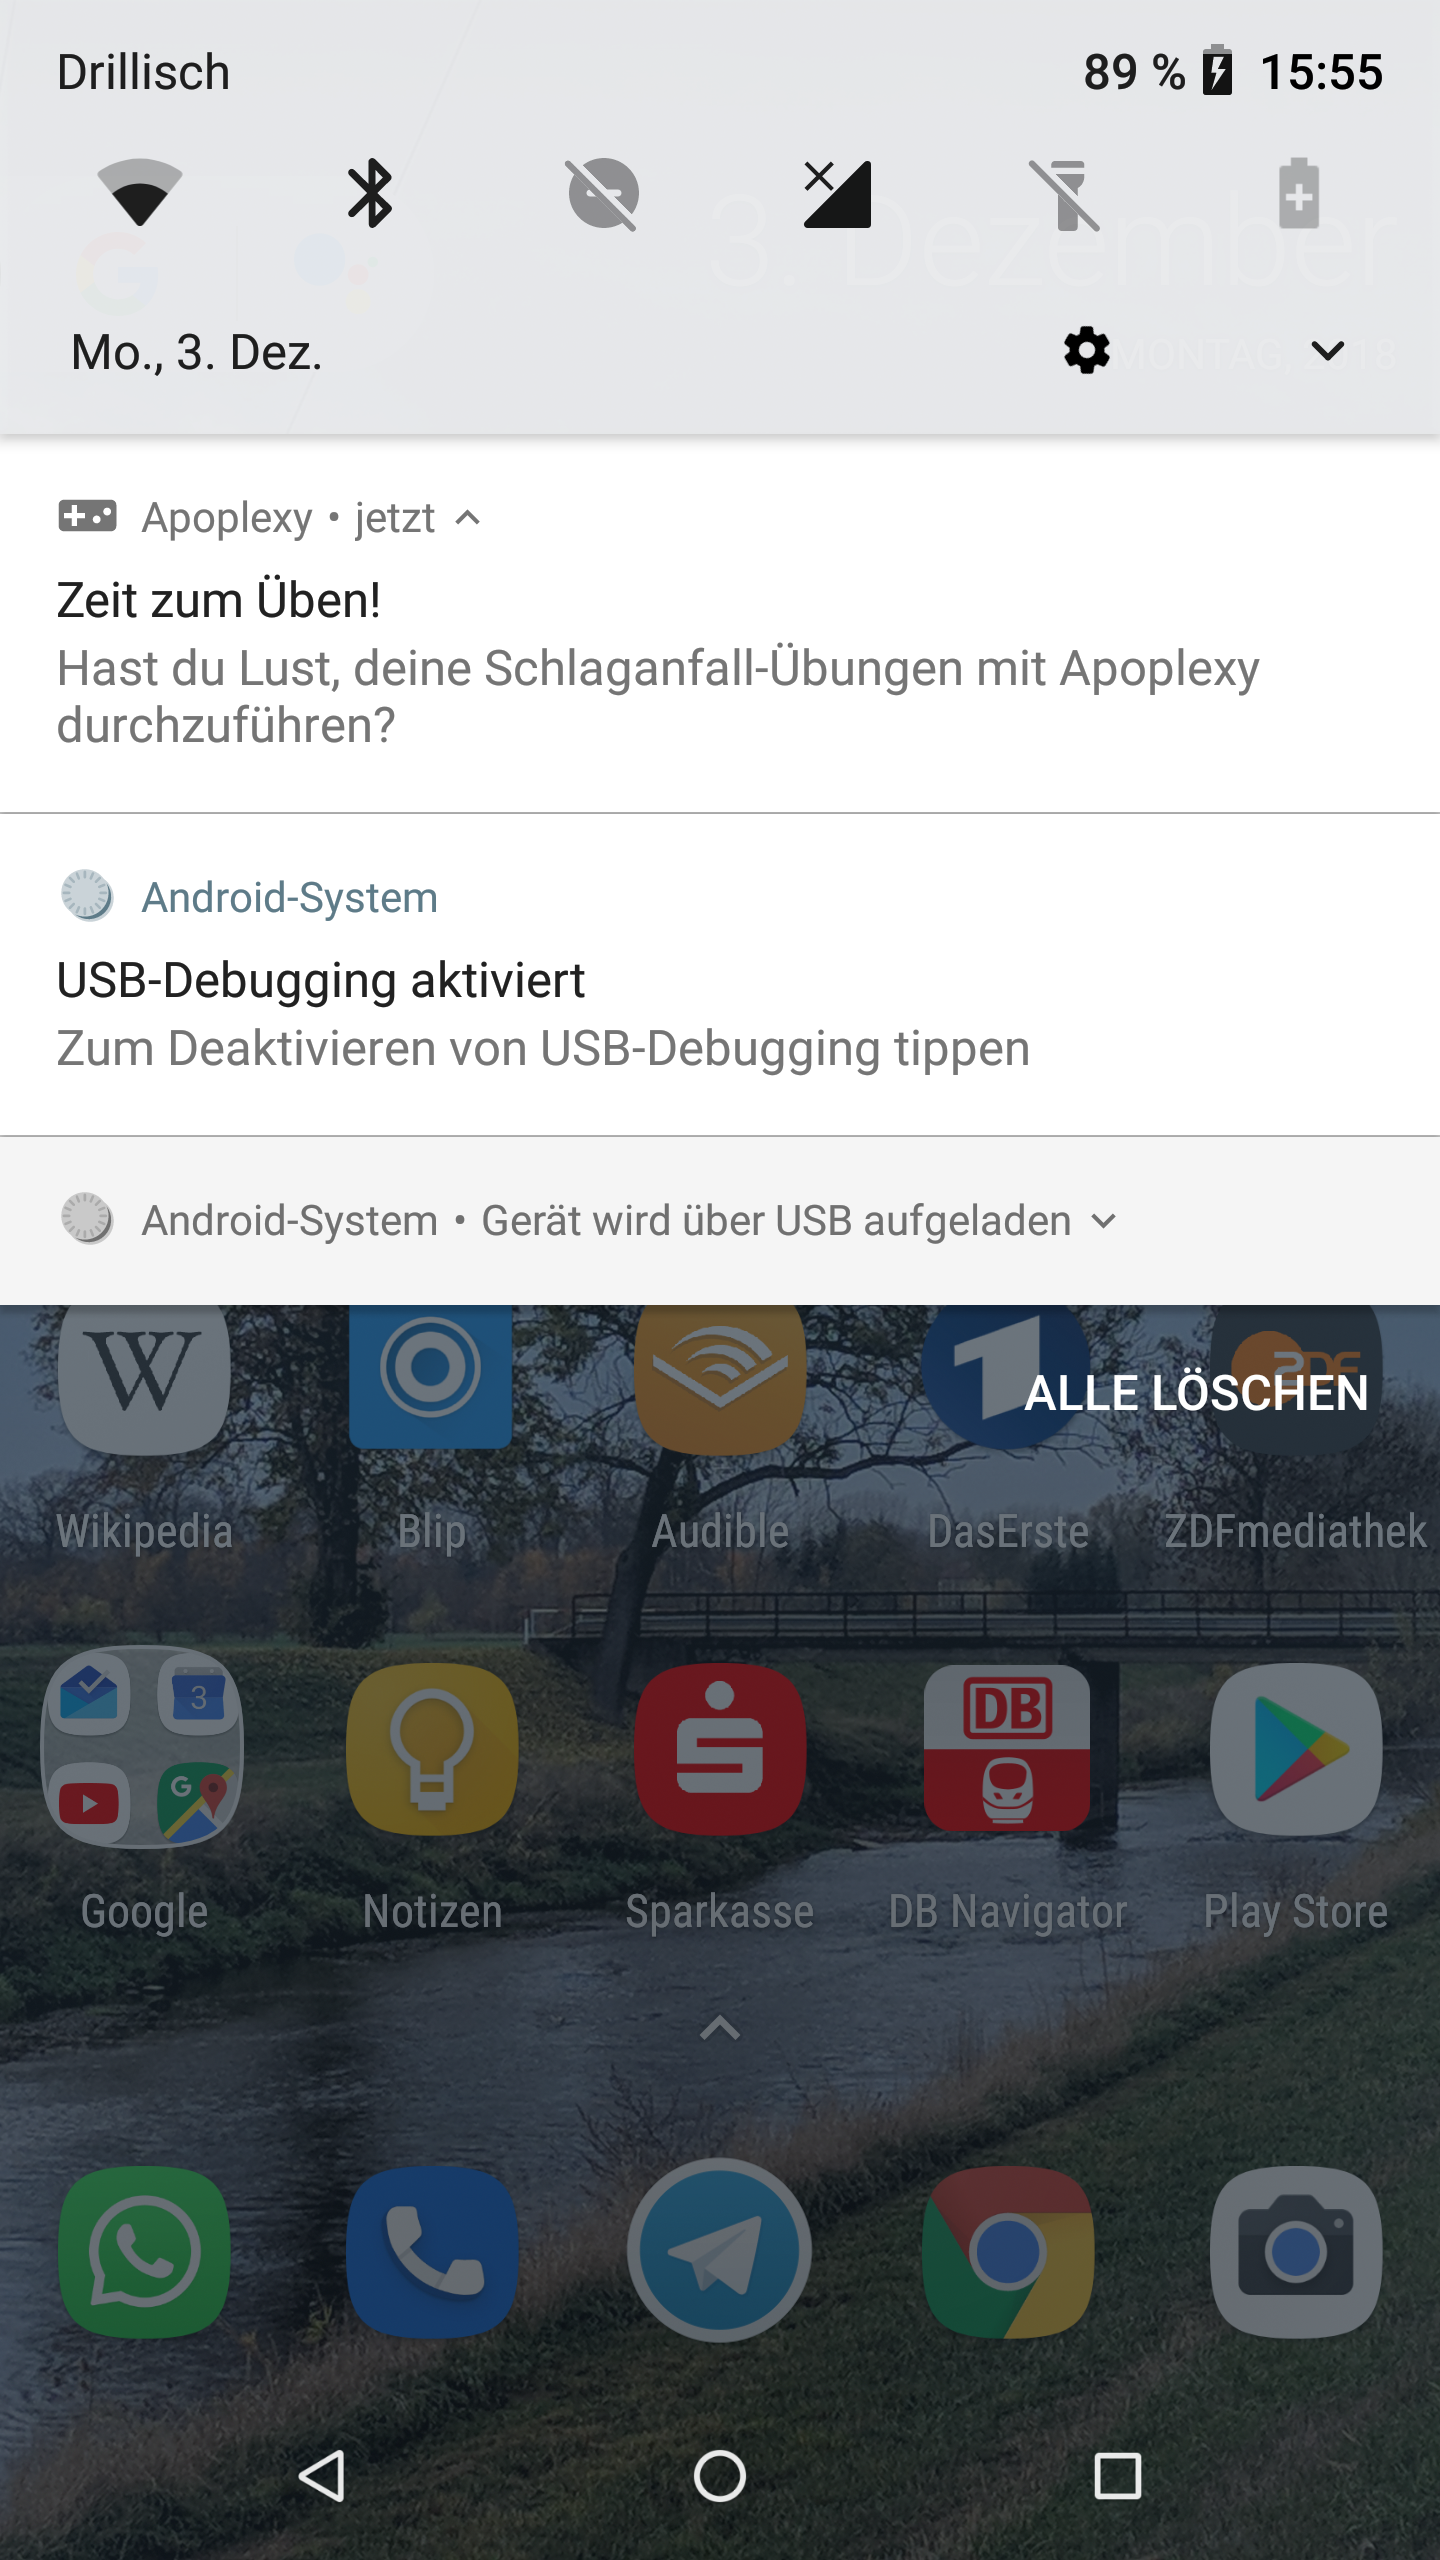
\includegraphics[scale=0.1]{pics/device-notification.png}
	\caption{Eine Übungsbenachrichtigung}
\end{figure}
\end{multicols}

\tocless\subsubsection{Kommunikation mit dem Mikrocontroller}
\begin{longlisting}
	\kotlinfile{../Softwareprodukt/App/app/src/main/java/de/lukasrost/apoplexy/BluetoothNoService.kt}
	\caption{Die \texttt{BluetoothNoService}-Klasse mit der Bluetooth-Funktionalität}
	\label{listing:bluetooth}
\end{longlisting}

\tocless\subsubsection{Konzept und programmiertechnische Umsetzung des Minispiels}
\begin{longlisting}
	\kotlinfile{../Softwareprodukt/App/app/src/main/java/de/lukasrost/apoplexy/game/PlaneGameView.kt}
	\caption{Die \texttt{PlaneGameView}-Klasse mit der Implementierung des Minispiels}
	\label{listing:game}
\end{longlisting}

\tocless\subsubsection{Umsetzung der Gamification in der App}
\begin{longlisting}
	\kotlinfile{../Softwareprodukt/App/app/src/main/java/de/lukasrost/apoplexy/helpers/GamificationGraderHelper.kt}
	\caption{Die \texttt{GamificationGraderHelper}-Klasse mit den Gamification-Bewertungsfunktionen}
	\label{listing:gamification}
\end{longlisting}